\chapter{Experimentación con modelos}\label{ap:experimentos}

Este anexo detalla los experimentos resumidos en la \cref{experimentaciuxf3n-con-modelos}. Como allí se advierte, los modelos no son directamente comparables entre sí: cada uno fue construido bajo criterios y premisas propios, con formatos de salida distintos, de modo que sus métricas no admiten una lectura como un ranking de desempeño. El propósito de esta etapa fue determinar qué manera de plantear el problema resulta más adecuada para un sistema de alerta temprana y qué enseñanzas deja cada intento sobre la naturaleza del fenómeno.

\section{LightGBM para intervalos de predicción}\label{lightgbm-para-intervalos-de-predicciuxf3n.}

El primer modelo consiste en un \lightgbm{} entrenado para pronosticar la cantidad de víctimas. La idea de este modelo es mostrar una línea temporal con la cantidad histórica de víctimas y, a partir del momento actual, una línea con el pronóstico esperado junto con los cuantiles \qty{10}{\percent} y \qty{90}{\percent}, que corresponden respectivamente al escenario de riesgo mínimo y al de riesgo máximo.

Durante el entrenamiento se crearon variables intermedias para mejorar el rendimiento del modelo, entre ellas \var{baseline\_60}, promedio de los últimos 60 días, y \var{promedio\_7dias}, promedio de los últimos siete días. El modelo predice 28 bloques de seis horas, es decir que su horizonte de predicción es de siete días.

\begin{table}[htbp]
\centering
\caption{Métricas de rendimiento del modelo LightGBM híbrido L1}
\label{tab:metricas-de-rendimiento-del-modelo-final}
\begin{tabularx}{\linewidth}{@{}>{\raggedright\arraybackslash}p{0.30\linewidth}c>{\raggedright\arraybackslash}X@{}}
\toprule
\textbf{Métrica de error} & \textbf{Valor} & \textbf{Interpretación} \\
\midrule
MAE (Error Absoluto Medio) & 0,9741 & Desviación promedio en valor absoluto entre la predicción y el valor observado. \\
\bottomrule
\end{tabularx}
\notaflot{Métricas calculadas sobre el conjunto de prueba.}
\end{table}

\begin{figure}[htbp]
\centering
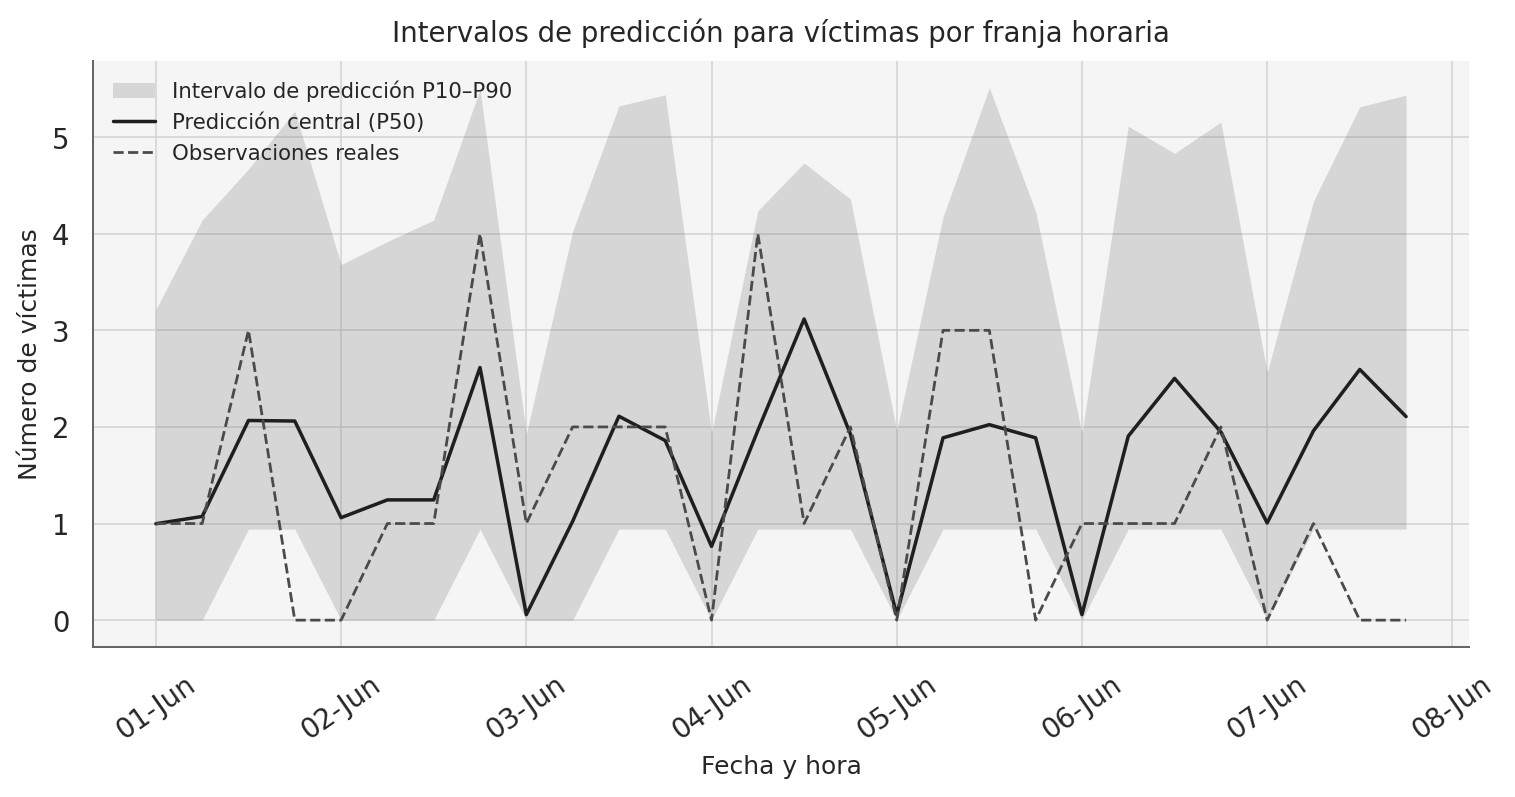
\includegraphics[width=\linewidth]{imagenes/image20.png}
\caption{Pronóstico con LightGBM: predicción central e intervalos P10--P90}
\label{fig:forecasting-lightgbm}
\notaflot{\fuentepropia{}.}
\end{figure}

En la \cref{fig:forecasting-lightgbm} se observa que, si bien el modelo no se ajusta perfectamente a la realidad, logra identificar cuándo ocurrirán incrementos o descensos en la cantidad de víctimas en toda la ciudad. Este hallazgo sugiere que los datos le permiten a \lightgbm{} aprender patrones de tendencia, y que enriquecerlos con más contexto puede mejorar el ajuste del pronóstico.

\section{Clasificador con perceptrón multicapa}\label{clasificador-con-perceptruxf3n-multicapa}

Este experimento busca establecer si plantear el problema como una clasificación de escenarios facilita a una red neuronal (perceptrón multicapa) alcanzar un buen desempeño. Para ello se generan tres categorías a partir de las necesidades del MPF: bajo, para dos víctimas o menos; medio, para hasta cuatro víctimas; y alto, a partir de cinco víctimas en un mismo bloque horario. Los resultados se presentan en la \cref{tab:metricas-de-desempeno-multilayer-percept}.

\begin{table}[htbp]
\centering
\caption{Métricas de desempeño del clasificador de perceptrón multicapa}
\label{tab:metricas-de-desempeno-multilayer-percept}
\begin{tabular}{@{}lcccc@{}}
\toprule
 & \textbf{Precisión} & \textbf{Sensibilidad} & \textbf{F1} & \textbf{Soporte} \\
\midrule
Alto & 0,0909 & 0,0125 & 0,0220 & 80 \\
Bajo & 0,5598 & 0,9035 & 0,6913 & 311 \\
Medio & 0,3469 & 0,0994 & 0,1545 & 171 \\
\midrule
Exactitud & & & 0,5320 & 562 \\
Promedio macro & 0,3325 & 0,3385 & 0,2893 & 562 \\
Promedio ponderado & 0,4283 & 0,5320 & 0,4327 & 562 \\
\bottomrule
\end{tabular}
\notaflot{\fuentepropia{}.}
\end{table}

El F1 ponderado de 0,4327 es bajo e indica que el desempeño general no es bueno, especialmente en las clases menos frecuentes. La exactitud de 0,5320 tampoco es una señal de buen rendimiento, porque el modelo puede obtenerla prediciendo mayoritariamente la clase «bajo» (sensibilidad de 0,9035 en esa clase). Se concluye que segmentar el problema en tres clases no es suficiente para generar un sistema de alerta temprana útil, al menos en las condiciones actuales.

\section{XGBoost regresor con capa de decisión Z-Score}\label{xgboost-regresor-muxe1s-capa-de-decisiuxf3n-z-score}

El resultado anterior obliga a replantear el enfoque. Si generar tres categorías no alcanza para un buen rendimiento, se propone un modelo regresor que prediga la cantidad de víctimas y una capa de decisión posterior que indique al usuario el riesgo para ese contexto particular.

Se entrena un \xgboost{} con 2227 registros en el conjunto de entrenamiento y 557 en el de prueba. La capa de decisión compara la cantidad de víctimas predicha con el promedio histórico para el mismo día de la semana y franja horaria. Por ejemplo, si la predicción es de cinco víctimas para un viernes al mediodía, se compara ese valor con el promedio histórico de víctimas de todos los viernes al mediodía. Mediante el puntaje estándar (Z-Score) se mide cuán desviada está la predicción de ese promedio y, según esa brecha, se asigna la categoría baja, media o alta. Una ventaja destacable de este esquema es que la sensibilidad del sistema puede calibrarse variando los umbrales de $z$. Los resultados se presentan en la \cref{tab:metricas-error-xgb-zscore}.

\begin{table}[htbp]
\centering
\caption{Métricas de error del XGBoost regresor con capa Z-Score}
\label{tab:metricas-error-xgb-zscore}
\begin{tabularx}{\linewidth}{@{}>{\raggedright\arraybackslash}p{0.30\linewidth}c>{\raggedright\arraybackslash}X@{}}
\toprule
\textbf{Métrica de error} & \textbf{Valor} & \textbf{Interpretación} \\
\midrule
Devianza de Poisson & 1,6627 & Medida de ajuste para datos de conteo; los valores menores indican mejor ajuste. \\
MAE (Error Absoluto Medio) & 1,2996 & Desviación promedio entre la cantidad de víctimas predicha y la observada, en la unidad original. \\
MSE (Error Cuadrático Medio) & 2,8783 & Promedio de los errores elevados al cuadrado; penaliza con mayor peso las desviaciones grandes. \\
RMSE (Raíz del Error Cuadrático Medio) & 1,6966 & Error típico del modelo expresado en cantidad de víctimas. \\
\bottomrule
\end{tabularx}
\notaflot{Métricas calculadas sobre el conjunto de prueba, con independencia del umbral de clasificación. \fuentepropia{}.}
\end{table}

La \cref{fig:capa-de-decision-z-score-y-su-distribuci} presenta la distribución de los valores de $z$ sobre el conjunto de prueba junto con los dos puntos de corte que delimitan los tres niveles de alarma. El eje horizontal expresa cuánto se desvía la predicción respecto del promedio histórico del mismo día de la semana y franja horaria, medido en desvíos estándar; el eje vertical representa la densidad de casos.

\begin{figure}[htbp]
\centering
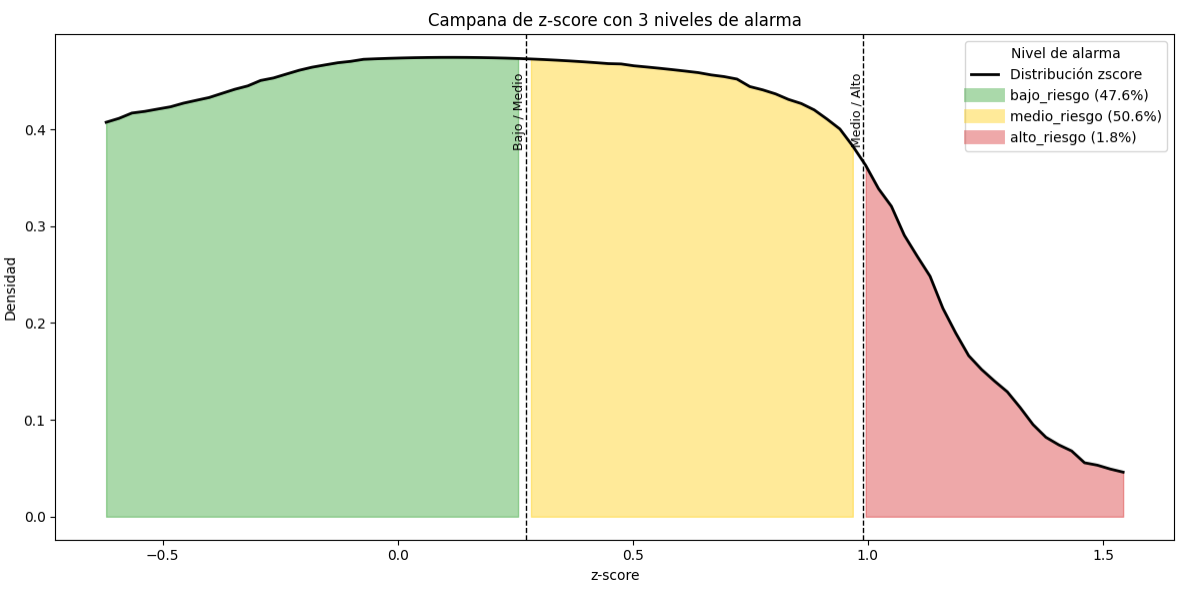
\includegraphics[width=\linewidth]{imagenes/image19.png}
\caption{Capa de decisión Z-Score y su distribución}
\label{fig:capa-de-decision-z-score-y-su-distribuci}
\notaflot{\fuentepropia{}.}
\end{figure}

El primer corte separa el nivel bajo del medio y el segundo, el medio del alto. La partición resultante ubica el \qty{47.6}{\percent} de los casos en riesgo bajo y el \qty{50.6}{\percent} en riesgo medio, mientras que el nivel alto queda reservado al \qty{1.8}{\percent} restante, correspondiente a la cola derecha de la distribución (\cref{tab:niveles-riesgo-zscore}). Esta asimetría es deliberada: el nivel alto está pensado para señalar situaciones excepcionales, y un umbral más permisivo multiplicaría las alertas máximas hasta volverlas rutinarias, con el consiguiente efecto de fatiga sobre el usuario. La principal ventaja del esquema es que ambos cortes son parámetros del sistema y no del modelo, de modo que pueden ajustarse según el criterio operativo del destinatario sin necesidad de reentrenar.

\begin{table}[htbp]
\centering
\caption{Distribución de los niveles de riesgo asignados por la capa Z-Score}
\label{tab:niveles-riesgo-zscore}
\begin{tabularx}{\linewidth}{@{}lX@{}}
\toprule
\textbf{Nivel de riesgo} & \textbf{Casos del conjunto de prueba} \\
\midrule
Bajo & \qty{47.6}{\percent} \\
Medio & \qty{50.6}{\percent} \\
Alto & \qty{1.8}{\percent} \\
\bottomrule
\end{tabularx}
\notaflot{Porcentajes calculados sobre el conjunto de prueba. \fuentepropia{}.}
\end{table}

Si bien las métricas no son plenamente satisfactorias, este modelo resulta de mayor utilidad que los anteriores. Puede mejorar si se exploran nuevas variables o con el aumento de la cantidad de datos para entrenar, y sus umbrales regulables permiten ajustar las alertas a la necesidad y al criterio del usuario final. Por esas razones se lo consideró seriamente para el producto mínimo viable.

\section{Perceptrón multicapa binario con capa de decisión}\label{perceptruxf3n-multicapa-binario-con-capa-de-decisiuxf3n.}

Considerando la metodología anterior, basada en una capa de decisión posterior a la predicción, se realiza un experimento para comprobar el desempeño de un perceptrón multicapa al emitir las alertas con esta configuración.

Las características del conjunto de datos son las mismas que en el \xgboost{} regresor, con el objetivo de aislar el efecto del modelo y conocer la contribución del perceptrón a la clasificación final. Varía, en cambio, la naturaleza del atributo objetivo, que es binario: el modelo produce una salida continua entre 0 y 1, sobre la cual se aplican cuantiles para clasificar.

\begin{table}[htbp]
\centering
\caption{Métricas del perceptrón multicapa binario con capa de decisión}
\label{tab:resumen-de-metricas-del-modelo}
\begin{tabular}{@{}lc@{}}
\toprule
\textbf{Métrica} & \textbf{Valor} \\
\midrule
AUC-ROC & 0,6289 \\
Puntaje de Brier & 0,2053 \\
\bottomrule
\end{tabular}
\notaflot{\fuentepropia{}.}
\end{table}

\section{XGBoost, modelo georreferenciado}\label{xgboost-modelo-georreferenciado}

Para que el modelo pase de ser solo temporal a espacio-temporal es necesario tomar algunas decisiones para adaptar la solución a la ciudad de Córdoba.

Inicialmente se propone una cuadrícula de 500~m por 500~m, en función del antecedente revisado \parencite{novello2022}. Luego de un análisis estadístico de distintos tamaños de cuadrícula y de la distribución de los siniestros en ellas, se determina que la configuración adecuada es una cuadrícula de 1000~m por 1000~m; si el modelo generaliza bien, el tamaño puede reducirse y evaluarse nuevamente.

Con la ciudad dividida en esa cuadrícula y cada día dividido en cuatro bloques de seis horas, cada combinación de celda y bloque horario constituye una fila del conjunto de datos. Teniendo en cuenta que la ciudad tiene 576~km\textsuperscript{2}, los registros totalizan 1.472.000 filas, de las cuales solo el \qty{0.28}{\percent} tiene accidentes. Esta es la dificultad central del problema: un modelo que siempre predijera que no va a pasar nada acertaría el \qty{99.7}{\percent} de las veces. La \cref{fig:esquema-del-modelo-georreferenciado-impu} representa el proceso de entrenamiento.

\begin{figure}[htbp]
\centering
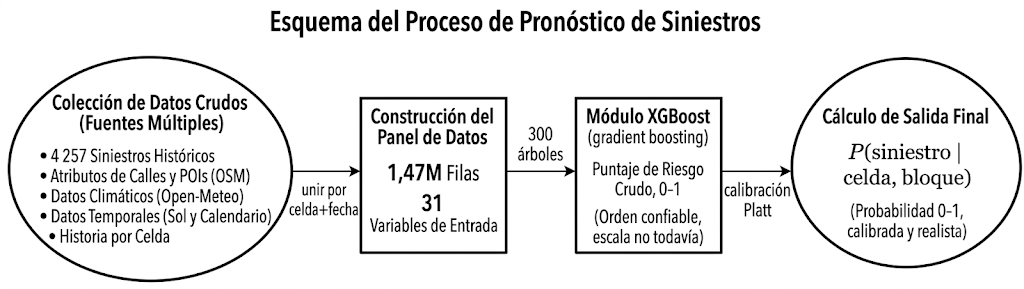
\includegraphics[width=\linewidth]{imagenes/image18.png}
\caption{Esquema del modelo georreferenciado impulsado por XGBoost}
\label{fig:esquema-del-modelo-georreferenciado-impu}
\notaflot{\fuentepropia{}.}
\end{figure}

Este modelo obtuvo resultados modestos frente al promedio histórico (PR-AUC de 0,0097 frente a 0,0085; ROC-AUC de 0,809 frente a 0,778), pero aportó información valiosa para la selección del modelo final. En síntesis, la forma correcta de evaluarlo es mediante validación \eng{walk-forward}; con pocos casos positivos conviene evitar la calibración isotónica y reemplazarla por el escalado de Platt; y el enfoque georreferenciado funciona (el modelo superó a la referencia en cinco validaciones distintas), por lo que tiene potencial de mejora si se continúan recolectando datos.

\section{AutoGluon-TimeSeries}\label{autogluon-timeseries}

En la etapa final de exploración se aplicó a los datos del problema el pipeline de aprendizaje automático automatizado de \autogluonts{}, ejecutado en el Centro de Computación de Alto Desempeño de la Universidad Nacional de Córdoba (CCAD-UNC). Como se explicó en el \cref{marco-teorico}, este paso permite entrenar varios modelos simultáneamente y obtener una combinación óptima.

Se configuró el predictor de series temporales de \autogluon{} para optimizar la métrica MASE sobre la variable objetivo en escala logarítmica (\var{victimas\_log}), con frecuencia de seis horas, estacionalidad diaria ($m = 4$) y un horizonte de predicción de 14 días (56 pasos), de manera de no perjudicar a modelos como DeepAR o TFT. Se definieron como covariables conocidas variables de calendario y contexto (\var{dia\_semana\_cat}, \var{es\_fin\_de\_semana}, \var{mes} y \var{tipomesESCOLAR}). El entrenamiento se ejecutó con el perfil \var{high\_quality}, con un tiempo total de 12 horas y una validación cruzada temporal (\eng{walk-forward}) de cuatro ventanas consecutivas.

\begin{table}[htbp]
\centering
\caption{Resultado del proceso de ensamble ponderado de AutoGluon}
\label{tab:resultado-del-proceso-de-ensamble-ponder}
\begin{tabular}{@{}lcccc@{}}
\toprule
\textbf{Modelo} & \textbf{Score prueba} & \textbf{Score validación} & \textbf{T. predicción} & \textbf{T. ajuste} \\
\midrule
Direct Tabular & $-0{,}6983$ & $-0{,}8229$ & 0,11 & 4,32 \\
DeepAR & $-0{,}7011$ & $-0{,}8143$ & 9,30 & 117,78 \\
Weighted Ensemble & $-0{,}7116$ & $-0{,}7823$ & 13,17 & 1,66 \\
AutoETS & $-0{,}7252$ & $-0{,}8077$ & 4,25 & 72,69 \\
TFT & $-0{,}7314$ & $-0{,}7911$ & 0,40 & 416,63 \\
\bottomrule
\end{tabular}
\notaflot{Los valores de score corresponden a la métrica MASE invertida (multiplicada por $-1$), donde los valores más cercanos a 0 indican mejor rendimiento. Los tiempos de predicción y de ajuste están expresados en segundos.}
\end{table}

El mejor desempeño corresponde a Direct Tabular, que en \autogluon{} agrupa modelos \xgboost{} o \lightgbm{} configurados con ventanas deslizantes. El resultado confirma las hipótesis con las que se desarrollaron los modelos anteriores y se alinea con los antecedentes citados en este trabajo.
